\section{Simulation Environment Implementation}

To ensure the safety of physical hardware and validate the multi-robot coordination logic, we constructed a high-fidelity simulation setup in Gazebo. This environment mirrors the physical cell's dimensions, kinematic properties, and sensor layout.

\subsection{Environment Composition}
The complete simulated workspace is illustrated in Figure~\ref{fig:full_gazebo_setup}. The environment was assembled by integrating distinct Unified Robot Description Format (URDF) and Xacro models into a unified Gazebo world.

\begin{figure}[H]
    \centering
    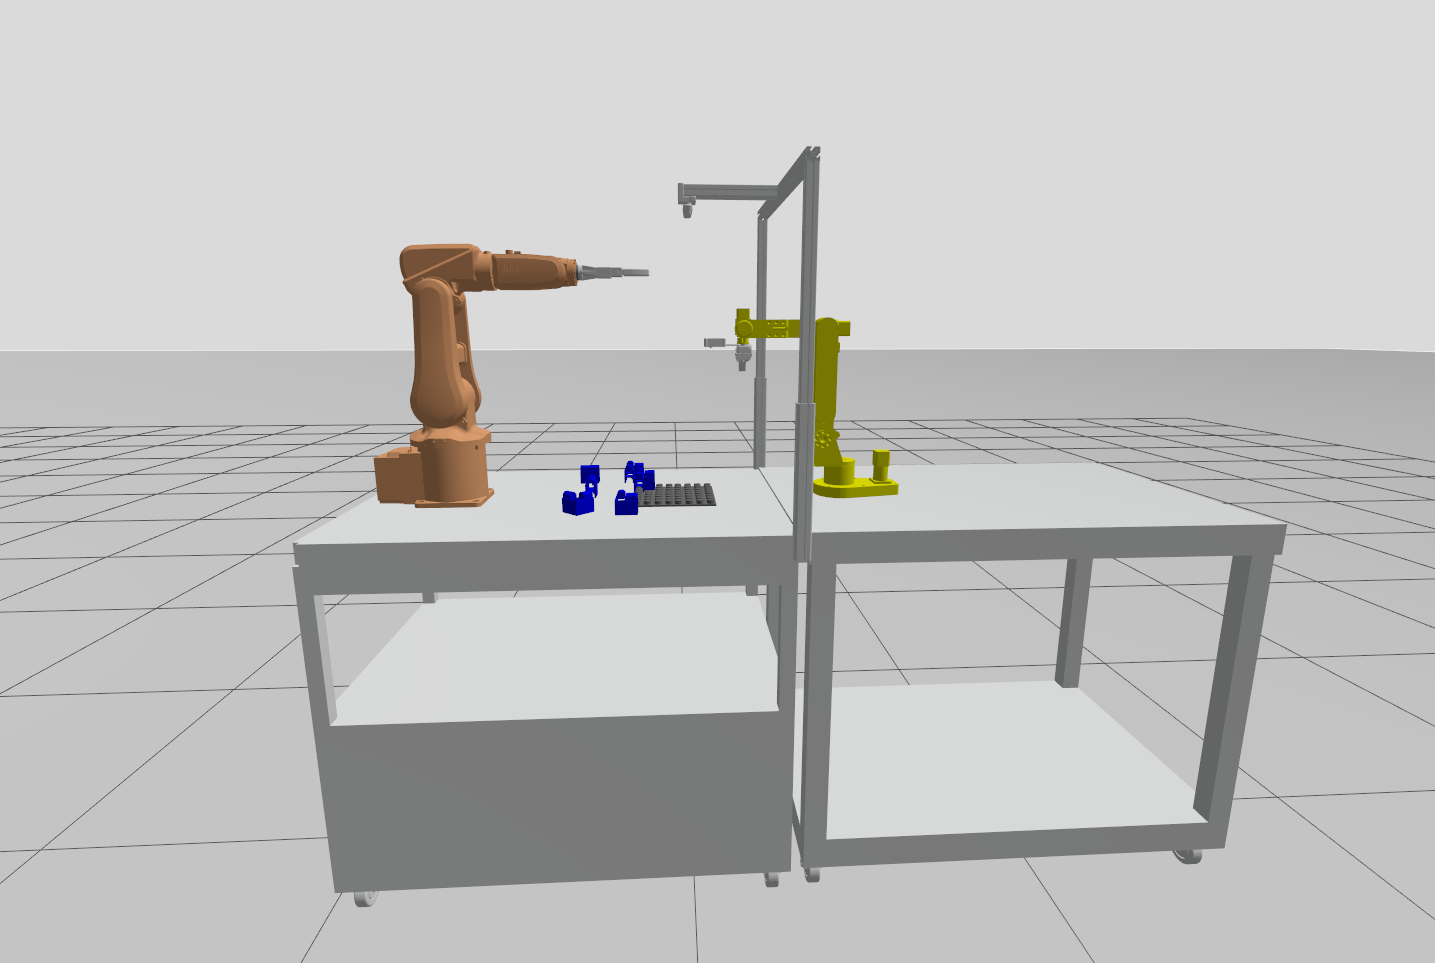
\includegraphics[width=0.7\textwidth]{Figures/chapter3/simulation/full_setup.png} % Replace with your full setup image file
    \caption{Overview of the complete Gazebo simulation environment, featuring the dual-robot cell, camera system, and assembly workspace.}
    \label{fig:full_gazebo_setup}
\end{figure}

Detailed breakdowns of the simulated components are presented in Figure~\ref{fig:sim_components}:

\begin{itemize}
    \item \textbf{Robotic Manipulators:} The ABB IRB120 and AR4 robots were imported using their respective Xacro macro definitions. Inertial properties and collision meshes were added to enabling accurate dynamic simulation via the Open Dynamics Engine (ODE).
    \item \textbf{Camera Stand:} A static model representing the physical aluminum extrusion stand was added to the world. This ensures the simulated sensor is positioned at the exact height and angle relative to the table as the real-world setup.
    \item \textbf{Workspace Objects:} The assembly table, the sorting grid, and the plastic bricks were modeled with dimensions identical to the physical setup. The bricks were assigned friction coefficients to mimic the plastic-on-table interaction.
\end{itemize}

% This block creates a 2x2 grid of your component pictures
\begin{figure}[H]
    \centering
    \begin{subfigure}[b]{0.45\textwidth}
        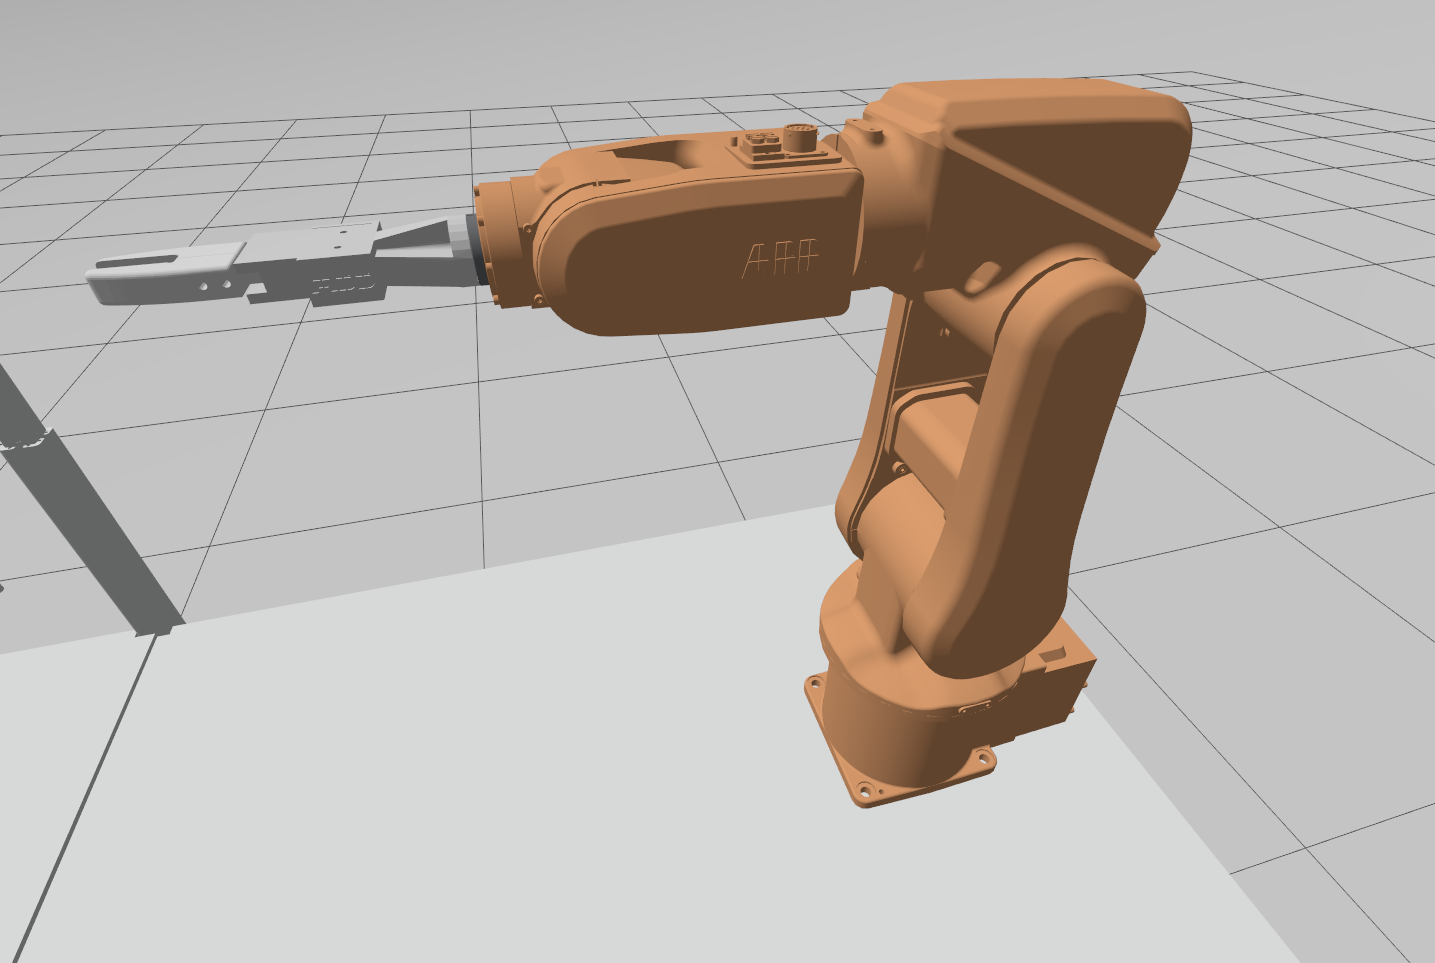
\includegraphics[width=\textwidth]{Figures/chapter3/simulation/abb_robot_simulation.png}
        \caption{ABB IRB120 Robot}
    \end{subfigure}
    \hfill
    \begin{subfigure}[b]{0.45\textwidth}
        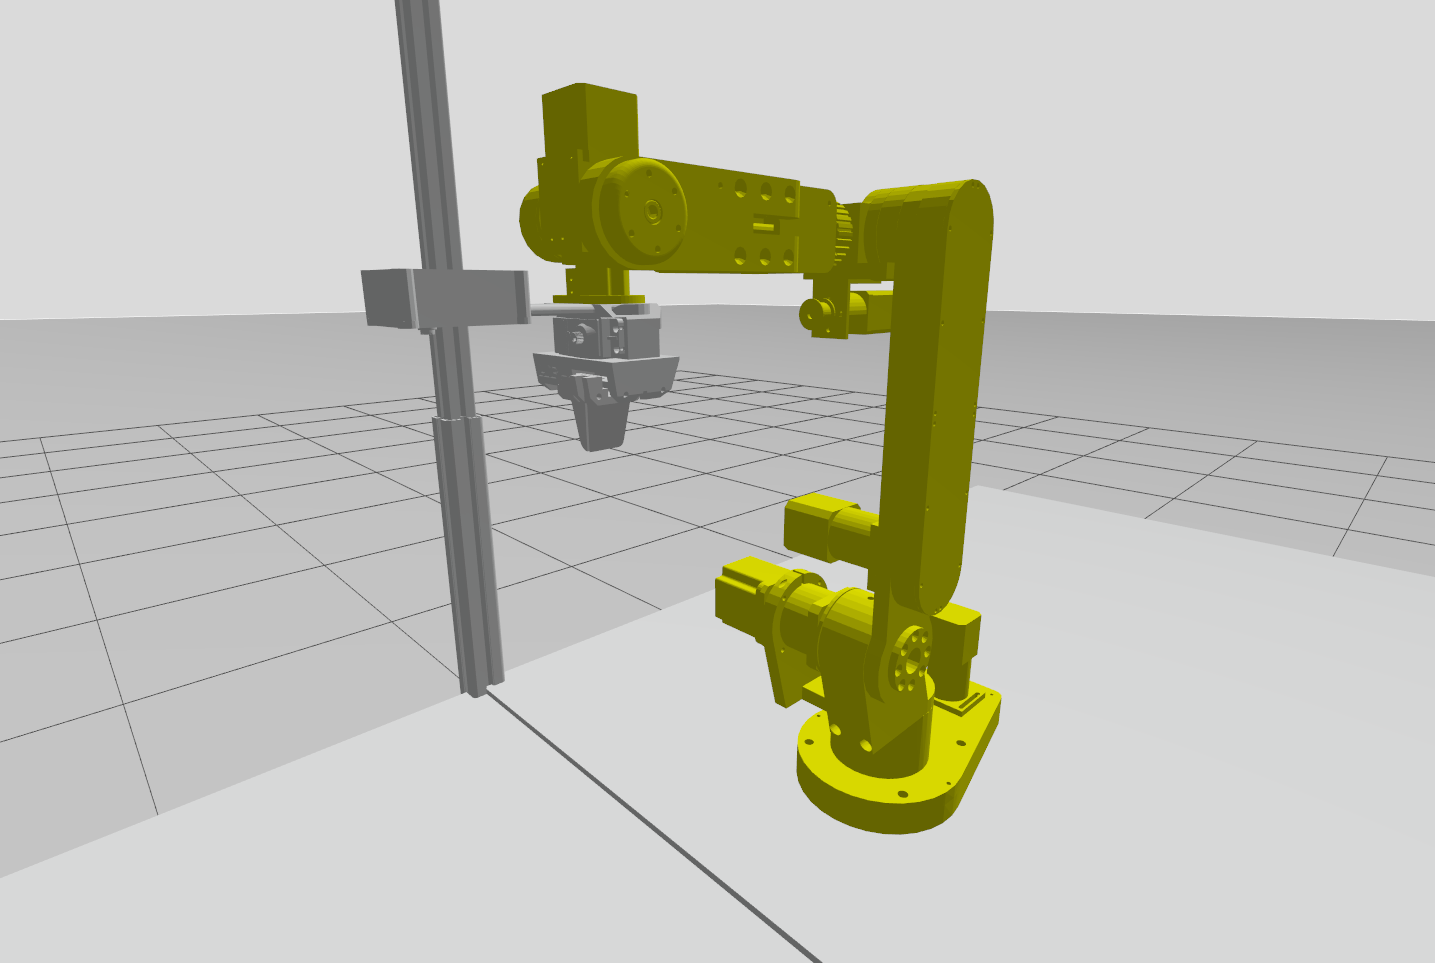
\includegraphics[width=\textwidth]{Figures/chapter3/simulation/ar4_simulation.png}
        \caption{AR4 Robot}
    \end{subfigure}
    
    \vspace{0.5cm} % Spacing between rows
    
    \begin{subfigure}[b]{0.45\textwidth}
        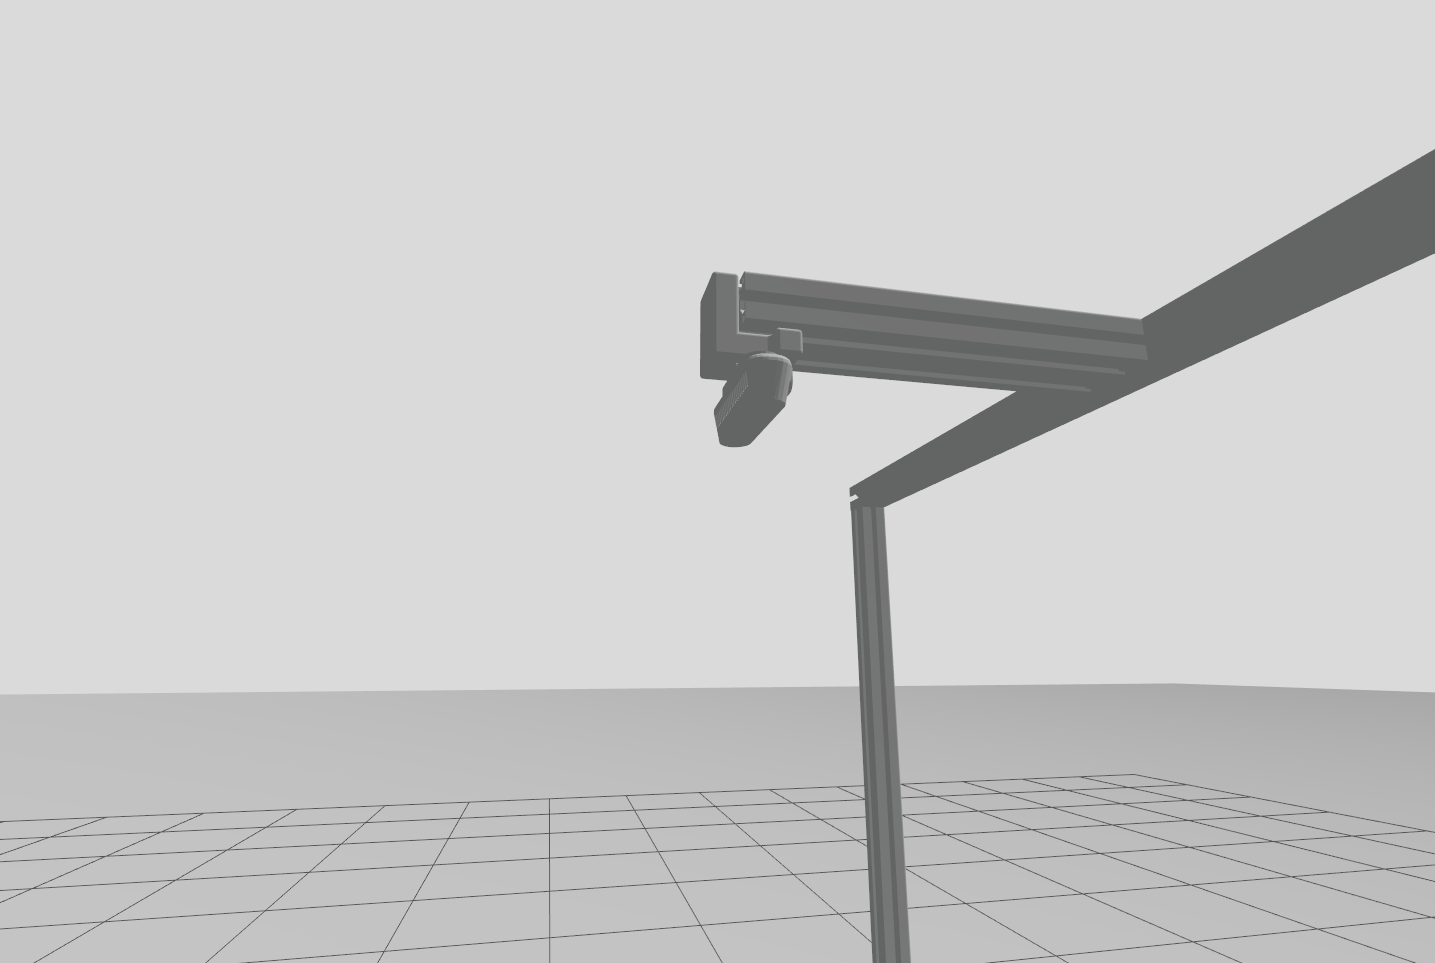
\includegraphics[width=\textwidth]{Figures/chapter3/simulation/camera_stand_simulation.png}
        \caption{Camera Stand}
    \end{subfigure}
    \hfill
    \begin{subfigure}[b]{0.45\textwidth}
        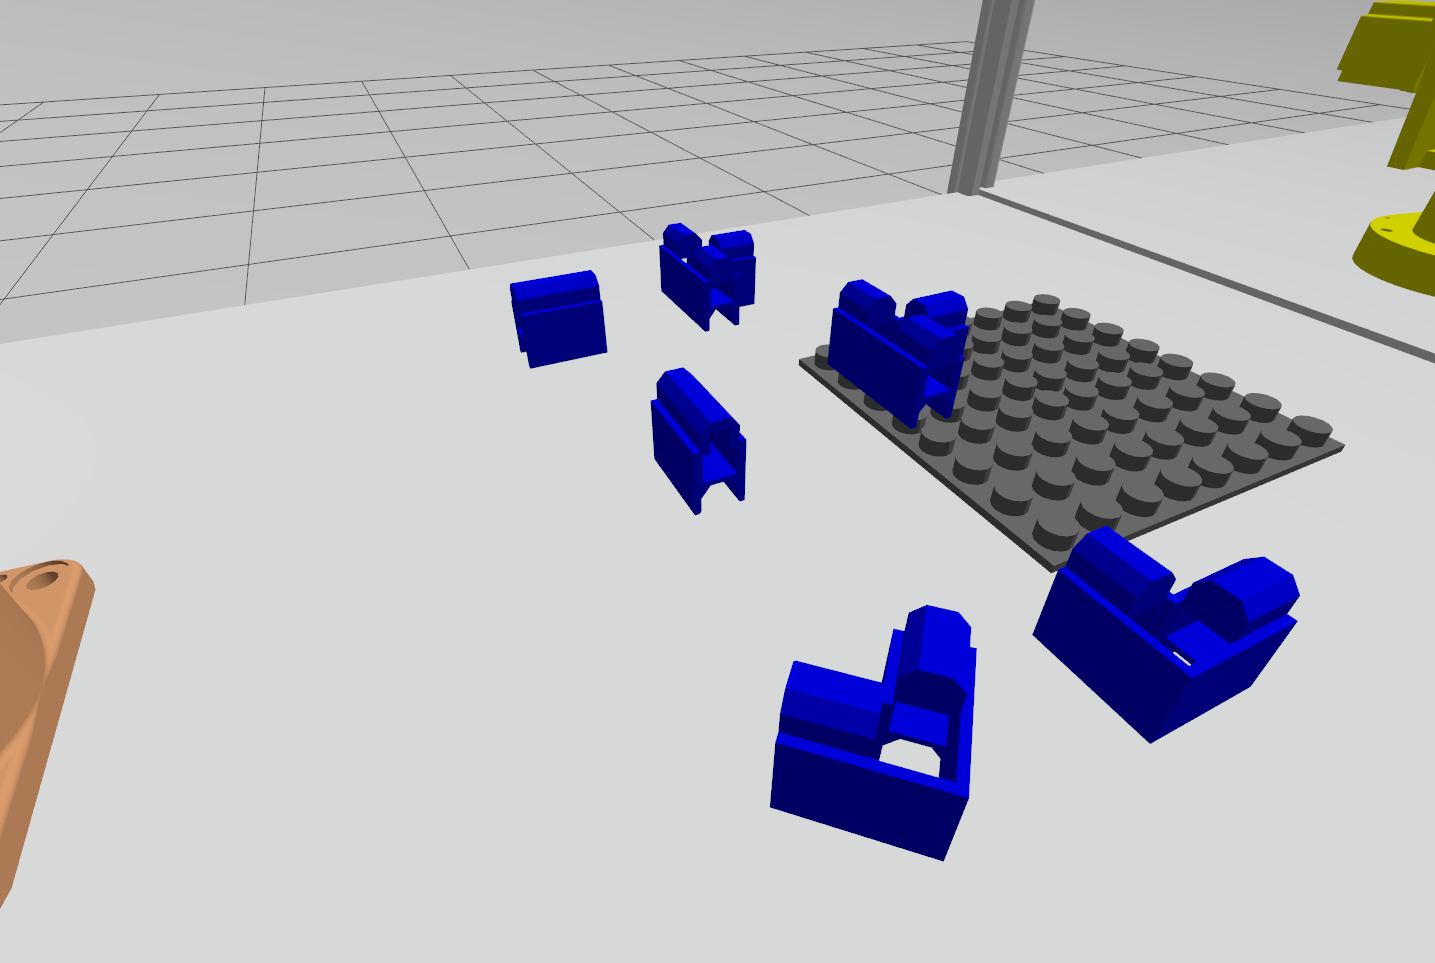
\includegraphics[width=\textwidth]{Figures/chapter3/simulation/bricks_grid.png}
        \caption{Bricks and Grid}
    \end{subfigure}
    \caption{Detailed component breakdown of the simulation environment.}
    \label{fig:sim_components}
\end{figure}

\clearpage

\subsection{Perception and Manipulation Verification}
\subsubsection{Synthetic Vision Feed}
To validate the computer vision pipeline, we utilized the \texttt{gazebo\_ros\_camera} plugin. Figure~\ref{fig:sim_camera_feed} displays the raw camera feed from the simulated sensor. The object colors in Gazebo were tuned to verify that the YOLO detection model function correctly before deployment.

\begin{figure}[H]
    \centering
    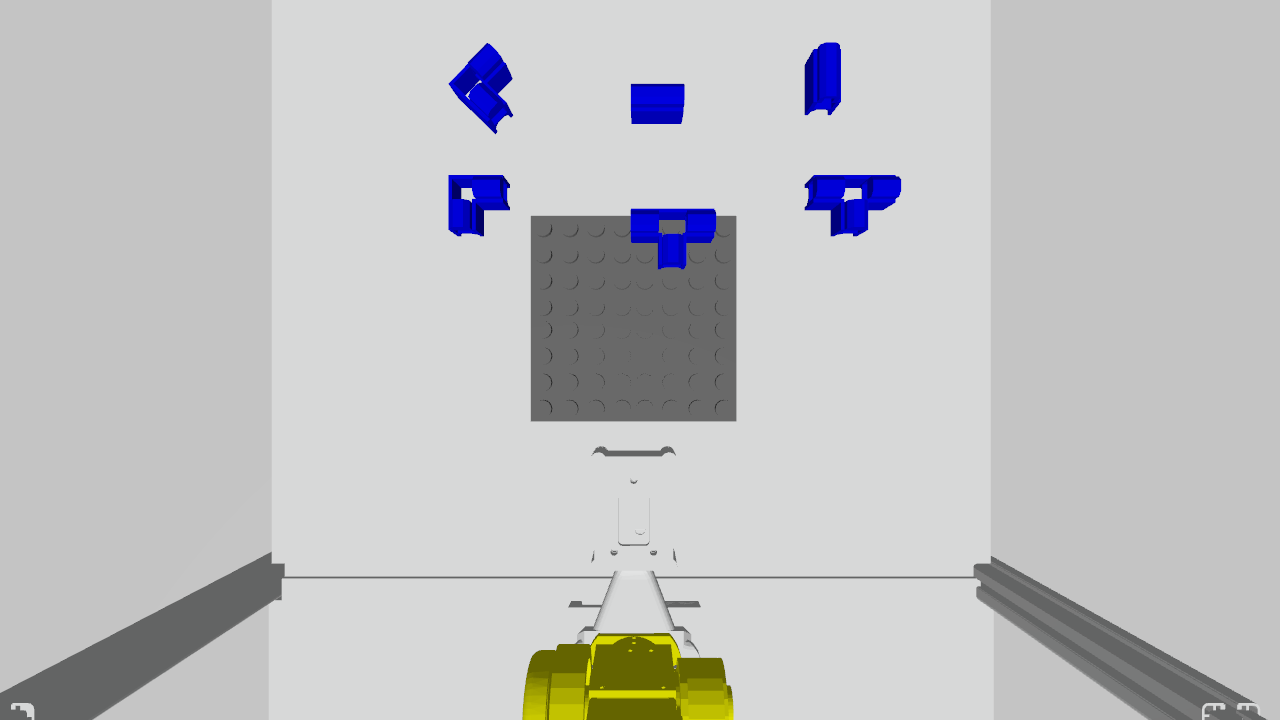
\includegraphics[width=0.7\textwidth]{Figures/chapter3/simulation/camera_feed_simulation.png} % Replace with your camera feed image
    \caption{Synthetic camera feed from the simulated RealSense sensor, demonstrating visibility of the bricks and grid.}
    \label{fig:sim_camera_feed}
\end{figure}

\subsubsection{Grasping Sequence Validation}
The kinematic reach and grasping logic were validated using the ABB IRB120. As shown in Figure~\ref{fig:abb_grasp_seq}, the robot successfully executes the pick sequence: approaching the detected brick, actuating the virtual gripper (via the Gazebo grasp plugin), and lifting the object without slippage.

% This block creates a strip of 3 images for the grasping sequence
\begin{figure}[H]
    \centering
    \begin{subfigure}[b]{0.32\textwidth}
        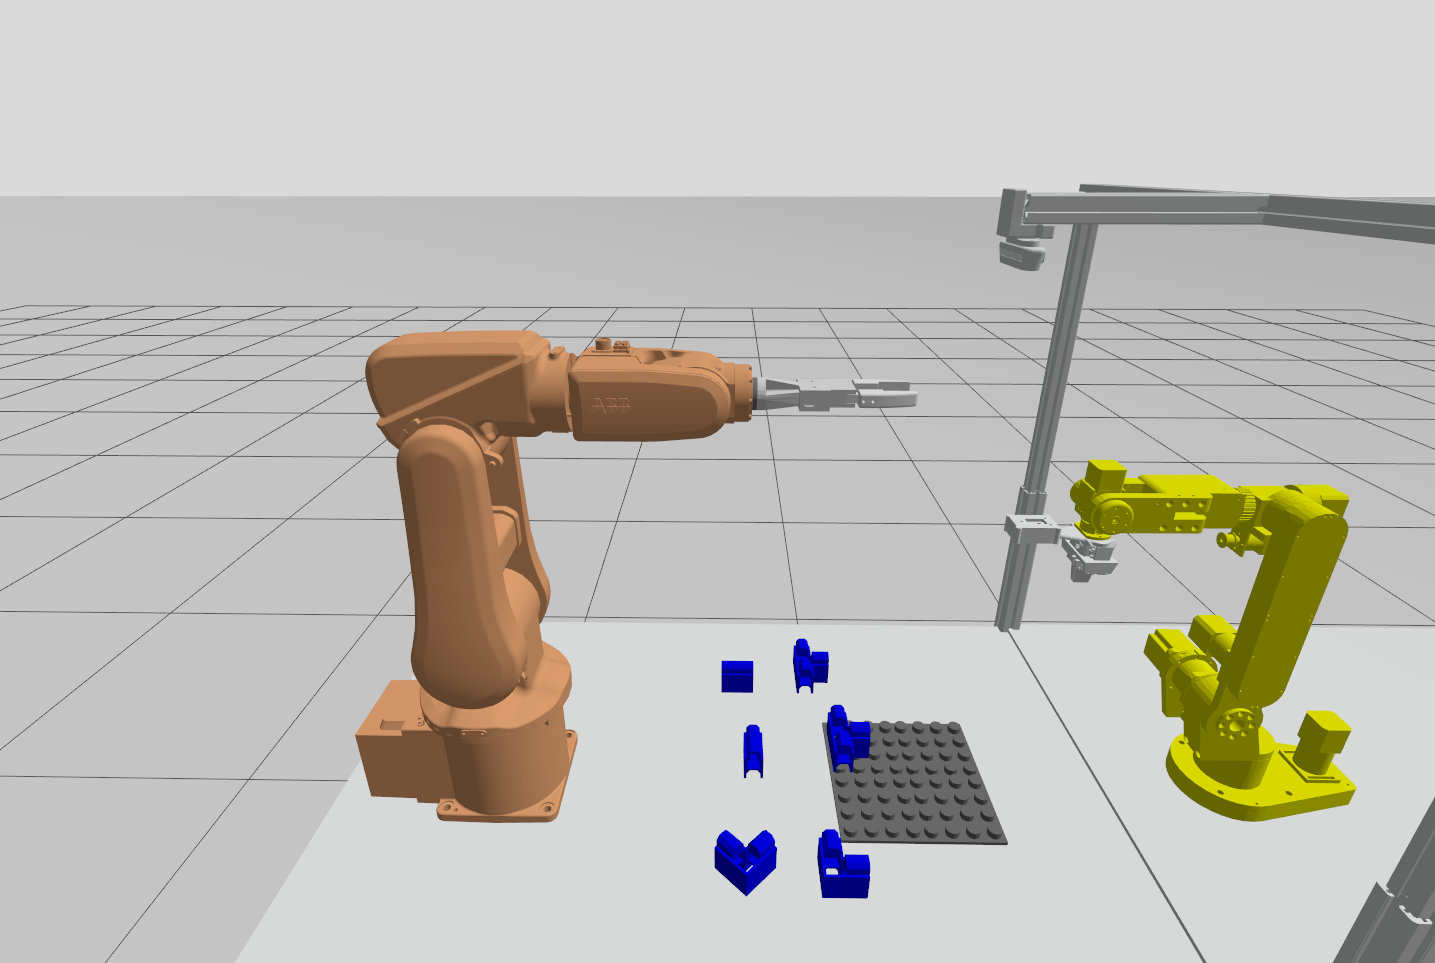
\includegraphics[width=\textwidth]{Figures/chapter3/simulation/grasp_1.png}
        \caption{Approach}
    \end{subfigure}
    \hfill
    \begin{subfigure}[b]{0.32\textwidth}
        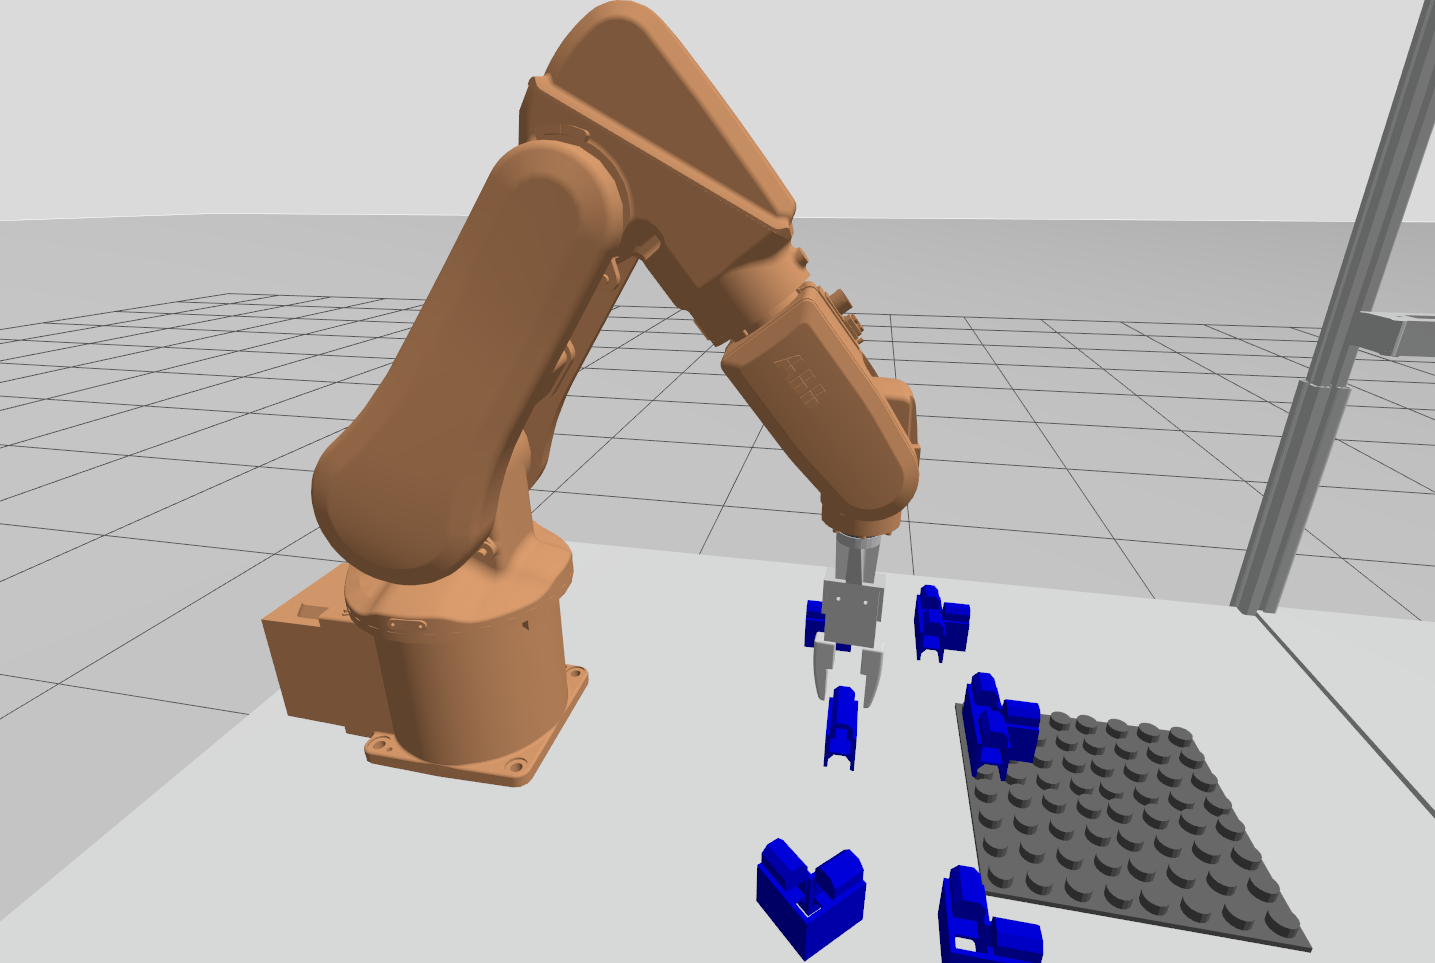
\includegraphics[width=\textwidth]{Figures/chapter3/simulation/grasp_2.png}
        \caption{Grasp Actuation}
    \end{subfigure}
    \hfill
    \begin{subfigure}[b]{0.32\textwidth}
        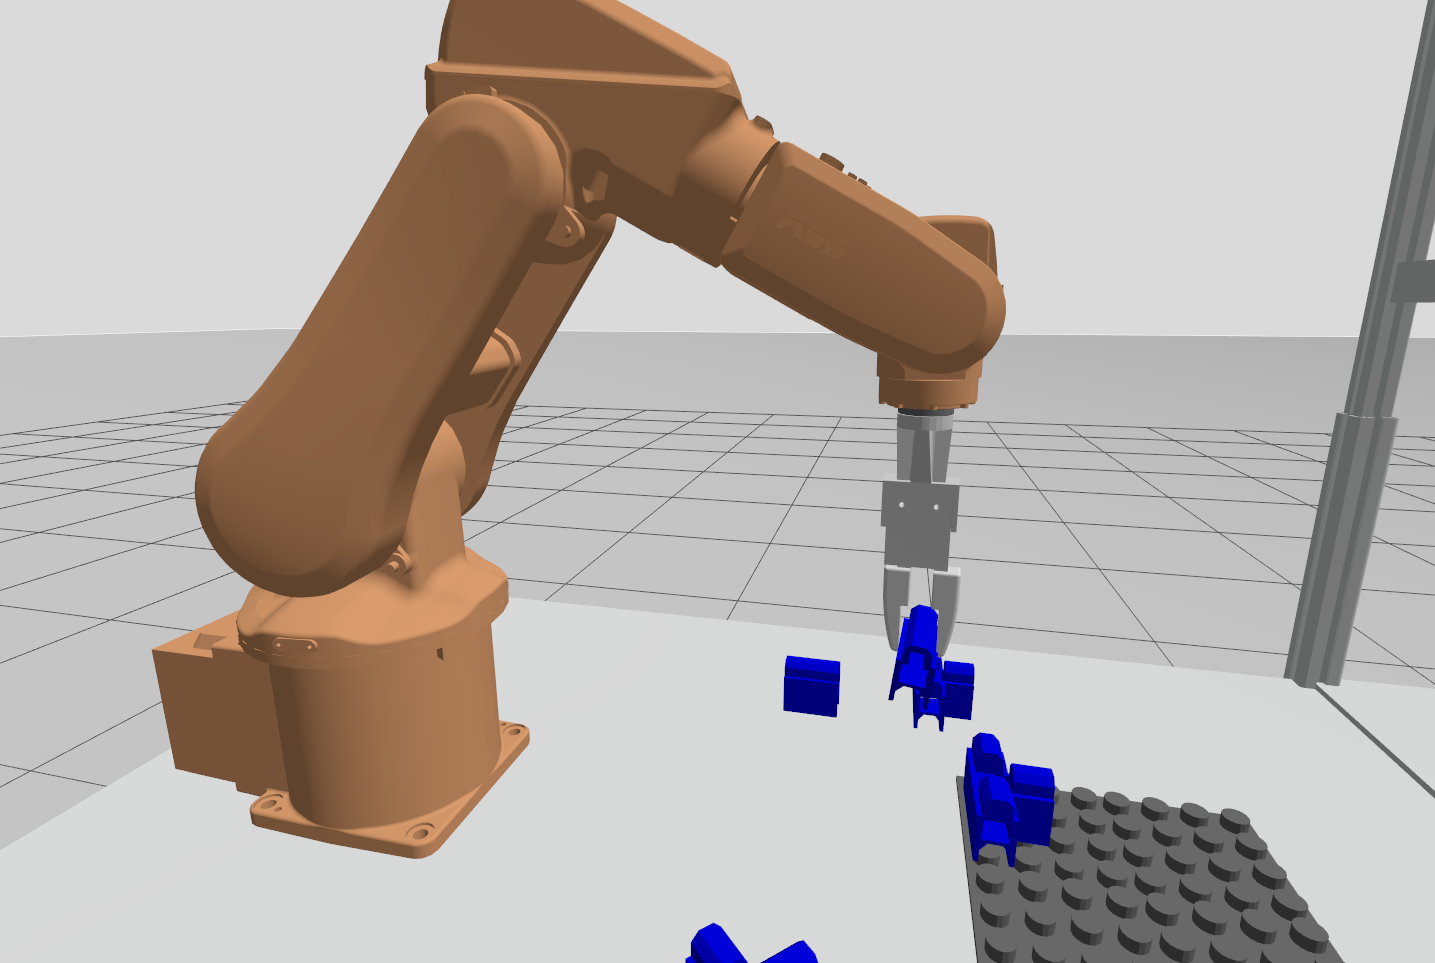
\includegraphics[width=\textwidth]{Figures/chapter3/simulation/grasp_3.png}
        \caption{Retract \& Lift}
    \end{subfigure}
    \caption{ABB IRB120 performing a successful pick operation in the simulation.}
    \label{fig:abb_grasp_seq}
\end{figure}